\documentclass[12pt,a4paper]{article}

% ─── PACKAGES ────────────────────────────────────────────────────────────────
\usepackage[utf8]{inputenc}
\usepackage[T1]{fontenc}
\usepackage{amsmath,amssymb}
\usepackage{graphicx}
\usepackage{xcolor}
\usepackage[margin=1in]{geometry}
\usepackage{tcolorbox}
\usepackage{enumitem}
\usepackage{tikz}
\usepackage{booktabs}
\usepackage{array}
\usepackage{tabularx}
\usepackage{colortbl}
\usepackage{mdframed}
\usepackage{titlesec}
\usepackage{titletoc}
\usepackage{fancyhdr}
\usepackage{hyperref}
\usepackage{multicol}
\usepackage{parskip}
\setlength{\headheight}{15pt}

\usetikzlibrary{shapes.geometric, arrows.meta, positioning, fit, backgrounds,
                decorations.pathreplacing, calc}

% ─── COLOUR PALETTE ──────────────────────────────────────────────────────────
\definecolor{navyblue}{RGB}{15,  52,  96}
\definecolor{royalblue}{RGB}{24,  90, 157}
\definecolor{skyblue}{RGB}{199, 228, 255}
\definecolor{accentcyan}{RGB}{0,  168, 204}
\definecolor{accentorange}{RGB}{230, 115,  0}
\definecolor{accentred}{RGB}{192,  36,  36}
\definecolor{accentgreen}{RGB}{30, 140,  70}
\definecolor{softgray}{RGB}{245, 247, 250}
\definecolor{midgray}{RGB}{180, 188, 200}
\definecolor{darkgray}{RGB}{60,  70,  85}
\definecolor{warmyellow}{RGB}{255, 214,  0}
\definecolor{paleyellow}{RGB}{255, 252, 220}
\definecolor{palegreen}{RGB}{220, 245, 225}
\definecolor{palered}{RGB}{255, 230, 230}
\definecolor{paleblue}{RGB}{230, 242, 255}

% ─── HYPERREF ────────────────────────────────────────────────────────────────
\hypersetup{
  colorlinks=true,
  linkcolor=royalblue,
  urlcolor=accentcyan,
  citecolor=accentorange,
  pdftitle={FROST-NS Technical Documentation},
  pdfauthor={NSS Team}
}

% ─── HEADER / FOOTER ─────────────────────────────────────────────────────────
\pagestyle{fancy}
\fancyhf{}
\fancyhead[L]{\small\color{midgray}\textit{FROST-NS Technical Documentation}}
\fancyhead[R]{\small\color{midgray}\textit{NSS Team}}
\fancyfoot[C]{\small\color{midgray}\thepage}
\renewcommand{\headrulewidth}{0.4pt}
\renewcommand{\headrule}{\hbox to\headwidth{\color{midgray}\leaders\hrule height \headrulewidth\hfill}}

% ─── SECTION STYLING ─────────────────────────────────────────────────────────
\titleformat{\section}
  {\Large\bfseries\color{navyblue}}
  {\colorbox{navyblue}{\textcolor{white}{\quad\thesection\quad}}}
  {0.8em}{}
  [\vspace{2pt}\color{accentcyan}\rule{\linewidth}{2pt}\vspace{4pt}]

\titleformat{\subsection}
  {\large\bfseries\color{royalblue}}
  {\thesubsection}
  {0.6em}{}
  [\vspace{1pt}\color{midgray}\rule{\linewidth}{0.6pt}]

\titleformat{\subsubsection}
  {\normalsize\bfseries\color{darkgray}}
  {\thesubsubsection}
  {0.5em}{}

% ─── TABLE OF CONTENTS ───────────────────────────────────────────────────────
\titlecontents{section}[2em]
  {\addvspace{4pt}\bfseries\color{navyblue}}
  {\contentslabel{2em}}{}
  {\dotfill\color{navyblue}\contentspage}

\titlecontents{subsection}[4.5em]
  {\addvspace{2pt}\small\color{darkgray}}
  {\contentslabel{2.5em}}{}
  {\dotfill\contentspage}

% ─── TCOLORBOX STYLES ────────────────────────────────────────────────────────
\tcbuselibrary{skins, breakable, listings}

% Problem / danger box
\newtcolorbox{problembox}[1][]{
  enhanced, breakable,
  colback=palered, colframe=accentred,
  fonttitle=\bfseries\small\color{white},
  coltitle=white, attach boxed title to top left={yshift=-2mm, xshift=4mm},
  boxed title style={colback=accentred, sharp corners},
  sharp corners=south, arc=4pt,
  title={#1},
  left=4pt, right=4pt, top=6pt, bottom=4pt
}

% Solution / info box
\newtcolorbox{solutionbox}[1][]{
  enhanced, breakable,
  colback=paleblue, colframe=royalblue,
  fonttitle=\bfseries\small\color{white},
  coltitle=white, attach boxed title to top left={yshift=-2mm, xshift=4mm},
  boxed title style={colback=royalblue, sharp corners},
  sharp corners=south, arc=4pt,
  title={#1},
  left=4pt, right=4pt, top=6pt, bottom=4pt
}

% Contribution / new feature box
\newtcolorbox{contribbox}[1][]{
  enhanced, breakable,
  colback=palegreen, colframe=accentgreen,
  fonttitle=\bfseries\small\color{white},
  coltitle=white, attach boxed title to top left={yshift=-2mm, xshift=4mm},
  boxed title style={colback=accentgreen, sharp corners},
  sharp corners=south, arc=4pt,
  title={#1},
  left=4pt, right=4pt, top=6pt, bottom=4pt
}

% Warning / TODO box
\newtcolorbox{warnbox}[1][]{
  enhanced, breakable,
  colback=paleyellow, colframe=accentorange,
  fonttitle=\bfseries\small\color{white},
  coltitle=white, attach boxed title to top left={yshift=-2mm, xshift=4mm},
  boxed title style={colback=accentorange, sharp corners},
  sharp corners=south, arc=4pt,
  title={#1},
  left=4pt, right=4pt, top=6pt, bottom=4pt
}

% Math equation highlight
\newtcolorbox{eqbox}{
  enhanced,
  colback=softgray, colframe=midgray,
  arc=6pt, left=8pt, right=8pt, top=6pt, bottom=6pt
}

% Phase boxes (for flowcharts)
\newtcolorbox{phasebox}[2][navyblue]{
  enhanced,
  colback=softgray, colframe=#1,
  fonttitle=\bfseries\small\color{white},
  coltitle=white,
  attach boxed title to top center={yshift=-2mm},
  boxed title style={colback=#1, rounded corners},
  arc=6pt,
  title={#2},
  left=6pt, right=6pt, top=8pt, bottom=6pt
}

% ─── INLINE BADGE ────────────────────────────────────────────────────────────
\newcommand{\newbadge}{\colorbox{accentgreen}{\tiny\color{white}\textbf{NEW}}\,}
\newcommand{\modbadge}{\colorbox{accentorange}{\tiny\color{white}\textbf{MOD}}\,}
\newcommand{\frombadge}{\colorbox{royalblue}{\tiny\color{white}\textbf{PAPER}}\,}
\newcommand{\contribbadge}{\colorbox{accentred}{\tiny\color{white}\textbf{OUR CONTRIBUTION}}\,}

% ─── TITLE PAGE ──────────────────────────────────────────────────────────────
\begin{document}

\begin{titlepage}
  
\begin{tikzpicture}[remember picture, overlay]
    % Top banner
    \fill[navyblue] (current page.north west) rectangle
      ([yshift=-5.5cm] current page.north east);
    % Accent stripe
    \fill[accentcyan] ([yshift=-5.5cm] current page.north west) rectangle
      ([yshift=-5.85cm] current page.north east);
    % Bottom bar
    \fill[softgray] (current page.south west) rectangle
      ([yshift=2.5cm] current page.south east);
    \fill[royalblue] ([yshift=2.5cm] current page.south west) rectangle
      ([yshift=2.85cm] current page.south east);
  \end{tikzpicture}

  \vspace*{5cm}
  {\color{blue}\centering
    {\fontsize{22}{26}\bfseries\selectfont
      Fatigue-Aware Risk Optimization\\[6pt]
      for Stochastic Task Allocation\\[6pt]
      in Nurse Scheduling}\par\vspace{10pt}
    {\large\color{accentcyan} A Comprehensive Technical Documentation}\par
  }

  \vfill
\end{titlepage}

% ─── TOC ─────────────────────────────────────────────────────────────────────
\tableofcontents
\newpage

% ─────────────────────────────────────────────────────────────────────────────
%  SECTION 1 · THE PROBLEM
% ─────────────────────────────────────────────────────────────────────────────
\section{The Problem}

\subsection{Business Context}

Hospitals face a critical challenge: \textbf{assigning nurses to shifts in the face of uncertain patient demand}. The core complexities are:

\begin{itemize}[leftmargin=18pt, itemsep=4pt]
  \item \textbf{Uncertain Demand} — Patient admissions fluctuate daily. A hospital must schedule nurses \emph{weeks in advance}, but doesn't know exact staffing needs until shifts occur.

  \item \textbf{Multiple Constraints} — Nurses have work-hour limits, shift-type preferences, rest requirements, fatigue thresholds, and availability windows. Management must balance these with cost.

  \item \textbf{Two Decision Points:}
    \begin{itemize}[itemsep=2pt]
      \item \textbf{Stage 1 (Now)} — Create a baseline schedule before knowing actual demand.
      \item \textbf{Stage 2 (Later)} — Adjust with emergency staff or cancelled shifts after demand is revealed.
    \end{itemize}

  \item \textbf{Cost Structure:}
    \begin{center}
      \begin{tabular}{lll}
        \toprule
        \textbf{Type} & \textbf{Cost/Nurse} & \textbf{When Used} \\
        \midrule
        Regular shift   & \$100 & Planned in advance \\
        Overtime shift  & \$150 & Planned, extra hours \\
        Emergency staff & \$200+ & Demand spike, last-minute \\
        \bottomrule
      \end{tabular}
    \end{center}

  \item \textbf{Patient Safety} — Fatigued nurses make medical errors. Scheduling recovery time costs money. This tradeoff is poorly understood and under-modelled.
\end{itemize}

\subsection{Mathematical Formulation}

Find an assignment of nurses $i \in I$ to shifts $k \in K$ on days $j \in J$ that minimises total cost across both stages:

\begin{eqbox}
\begin{equation}
\text{Minimize:}\quad
\underbrace{c_1 \textstyle\sum sr_{ijk}}_{\text{Regular cost}}
+\underbrace{c_2 \textstyle\sum so_{ijk}}_{\text{Overtime cost}}
+\underbrace{\mathbb{E}\bigl[q^{+}\alpha + q^{-}\beta\bigr]}_{\text{Expected recourse}}
\end{equation}
\end{eqbox}

\noindent Subject to:
\begin{align}
  \sum_k (sr_{ijk}+so_{ijk}) &\leq 1 \quad \forall i,j
    && \text{(one shift per day)}\\
  \sum_{j,k}(sr_{ijk}+so_{ijk}) &\leq n_1 \quad \forall i
    && \text{(max total shifts)}\\
  \sum_j(sr_{ijN}+so_{ijN}) &\leq n_2 \quad \forall i
    && \text{(max night shifts)}\\
  \sum_i(sr_{ijk}+so_{ijk}) + \alpha_{jk}^{\omega} - \beta_{jk}^{\omega}
    &\geq R_{jk}^{\omega}
    && \text{(demand fulfillment)}
\end{align}

\newpage
% ─────────────────────────────────────────────────────────────────────────────
%  SECTION 2 · THE PAIN POINTS
% ─────────────────────────────────────────────────────────────────────────────
\section{The Pain Points}

\begin{problembox}[Challenge 1 — Uncertain Demand]
Demand for nursing care is \textbf{stochastic and correlated}:
\begin{itemize}[itemsep=2pt]
  \item Traffic accidents increase ER admissions; seasonal flu waves stress the ICU.
  \item Weather and holidays shift patient flow in hard-to-predict ways.
\end{itemize}
Simple averages hide this variability, leading to:\\[4pt]
\begin{tabular}{@{}ll@{}}
  \textcolor{accentred}{\textbf{Under-staffing}} in high-demand scenarios & $\rightarrow$ poor patient care\\
  \textcolor{accentorange}{\textbf{Over-staffing}} in low-demand scenarios & $\rightarrow$ wasted payroll
\end{tabular}
\end{problembox}

\vspace{6pt}
\begin{problembox}[Challenge 2 — Nurse Fatigue \& Patient Safety]
Evidence shows fatigued nurses make significantly more errors:
\begin{itemize}[itemsep=2pt]
  \item Each additional shift increases error rate \emph{exponentially} (Jaber et al., 2013).
  \item Medical errors cost hospitals \$4,000–\$20,000 per incident.
\end{itemize}
Previous models either: ignore fatigue (unrealistic), use nonlinear models (intractable), or guess at parameters (unvalidated).
\end{problembox}

\vspace{6pt}
\begin{problembox}[Challenge 3 — Conflicting Objectives]
Three goals frequently contradict each other:
\begin{center}
\begin{tabular}{@{}lll@{}}
  \toprule
  \textbf{Goal} & \textbf{Action} & \textbf{Side-effect}\\
  \midrule
  Cost Minimisation & Use cheap regular shifts & Under-staffing in high demand\\
  Reliability & Cover all scenarios & Expensive emergency staffing\\
  Safety & Limit fatigue & More shifts needed, higher cost\\
  \bottomrule
\end{tabular}
\end{center}
No existing tool balances all three \emph{systematically}.
\end{problembox}

\vspace{6pt}
\begin{problembox}[Challenge 4 — Computational Complexity]
Problem size grows explosively:
\[
  30\text{ nurses} \times 30\text{ days} \times 4\text{ shifts} \times 20\text{ scenarios}
  = \mathbf{72{,}000}\text{ decision variables}
\]
Each constraint must hold per scenario, per day, per shift. Standard MIP solvers struggle without specialised decomposition techniques.
\end{problembox}

\newpage
% ─────────────────────────────────────────────────────────────────────────────
%  SECTION 3 · THE SOLUTION
% ─────────────────────────────────────────────────────────────────────────────
\section{The Solution: FROST-NS Framework}

\subsection{Overview}

\begin{solutionbox}[What FROST-NS Does]
\textbf{FROST-NS} (\textit{Fatigue-aware Risk Optimization for Stochastic Task allocation in Nurse Scheduling}) solves the nurse scheduling problem by combining four innovations into one coherent system:

\begin{enumerate}[itemsep=4pt]
  \item \textbf{Two-Stage Stochastic Optimisation} — Baseline decisions made now; adjustments made once demand is known.
  \item \textbf{CVaR Risk Control} — Limits worst-case shortages, not just the average.
  \item \textbf{Piecewise-Linear Fatigue Modelling} — Approximates exponential fatigue with \(<0.5\%\) error while staying MIP-solvable.
  \item \textbf{Advanced Constraint Library} — 22+ constraints covering night rest, weekends off, shift quotas, and soft penalties.
\end{enumerate}
\end{solutionbox}

\subsection{Our Contributions}

\subsubsection{Contribution 1 — Two-Stage Stochastic Programming \frombadge\modbadge}

\begin{center}
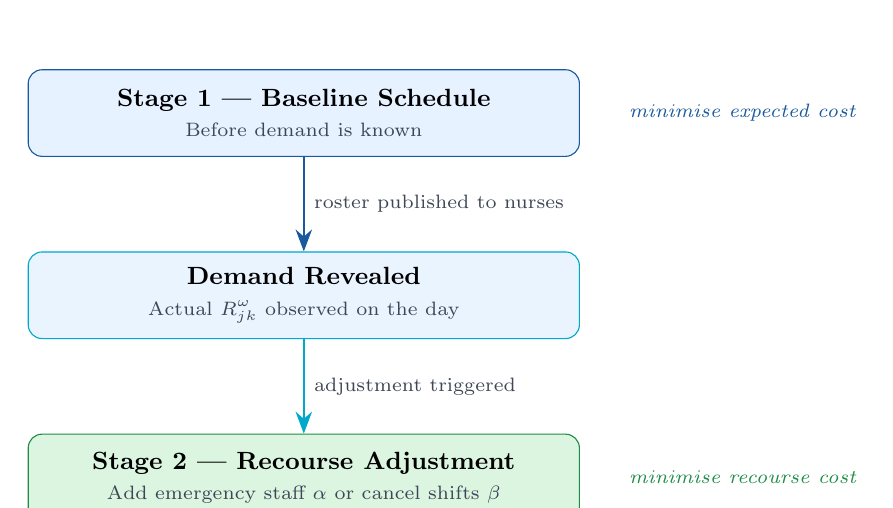
\begin{tikzpicture}[
  node distance=1.2cm,
  box/.style={draw, rounded corners=5pt, minimum width=7cm,
              minimum height=1.1cm, text centered, align=center, font=\small},
  arrow/.style={-{Stealth[scale=1.2]}, thick}
]
  \node[box, fill=paleblue, draw=royalblue] (s1)
    {\textbf{Stage 1 — Baseline Schedule}\\{\scriptsize\color{darkgray}Before demand is known}};
  \node[box, fill=skyblue!40, draw=accentcyan, below=of s1] (demand)
    {\textbf{Demand Revealed}\\{\scriptsize\color{darkgray}Actual $R_{jk}^{\omega}$ observed on the day}};
  \node[box, fill=palegreen, draw=accentgreen, below=of demand] (s2)
    {\textbf{Stage 2 — Recourse Adjustment}\\{\scriptsize\color{darkgray}Add emergency staff $\alpha$ or cancel shifts $\beta$}};

  \draw[arrow, royalblue] (s1) -- node[right, font=\scriptsize, color=darkgray]{roster published to nurses} (demand);
  \draw[arrow, accentcyan] (demand) -- node[right, font=\scriptsize, color=darkgray]{adjustment triggered} (s2);

  \node[right=0.5cm of s1,  font=\scriptsize\itshape\color{royalblue}]  {minimise expected cost};
  \node[right=0.5cm of s2,  font=\scriptsize\itshape\color{accentgreen}] {minimise recourse cost};
\end{tikzpicture}
\end{center}

\subsubsection{Contribution 2 — CVaR Risk Management \frombadge\modbadge}

\begin{solutionbox}[Why Expected Value Is Not Enough]
Minimising $\mathbb{E}[\text{shortage}]$ ignores tail risk. A 1000-shift shortage in 1\% of scenarios barely moves the average, but in practice it is catastrophic.

\textbf{CVaR fix:} ``What is the expected shortage in the \emph{worst 5\%} of scenarios?''
\end{solutionbox}

\begin{eqbox}
\begin{equation}
  \operatorname{CVaR}_{\sigma}[\text{Loss}]
  = \mathbb{E}\bigl[\text{Loss} \mid \text{Loss} \geq \operatorname{VaR}_{\sigma}\bigr]
  \quad \leq \;\mu
\end{equation}
\end{eqbox}

\subsubsection{Contribution 3 — Fatigue Dynamics via McCormick Linearisation \contribbadge}

\textbf{The problem in plain words.} Fatigue does not just grow — it also recovers. A nurse who works today decays slowly (only 12 hours of rest between shifts). A nurse who is off today decays faster (24 hours of rest). This means the decay rate in the fatigue update equation depends on whether the nurse works. Mathematically, this creates a product of two variables:

\begin{eqbox}
\[
  F_{i,j-1} \;\times\; w_{i,j}
\]
where $F_{i,j-1}$ is yesterday's fatigue (a continuous number) and $w_{i,j}$ is a binary variable equal to 1 if the nurse works today and 0 if she is off.
\end{eqbox}

Multiplying a continuous variable by a binary variable is \textbf{nonlinear}. Standard MIP solvers cannot handle this directly. We need to rewrite it as something linear.

\vspace{6pt}
\textbf{The fix — McCormick auxiliary variable.} We introduce a helper variable $fw_{i,j}$ and declare that it \emph{represents} the product $F_{i,j-1} \times w_{i,j}$. We then add three linear constraints that force the solver to set $fw_{i,j}$ to the correct value automatically:

\begin{eqbox}
\begin{align}
  fw_{i,j} &\leq M \cdot w_{i,j} \tag{MC1}\\
  fw_{i,j} &\leq F_{i,j-1} \tag{MC2}\\
  fw_{i,j} &\geq F_{i,j-1} - M(1 - w_{i,j}) \tag{MC3}\\
  fw_{i,j} &\geq 0 \tag{MC4}
\end{align}
where $M = F_{\max} = 0.70$ (the tightest possible upper bound on fatigue).
\end{eqbox}

\textbf{Why this works — two cases:}

\begin{center}
\begin{tabularx}{\textwidth}{@{}lXX@{}}
  \toprule
  & \textbf{Nurse is OFF} ($w_{i,j}=0$) & \textbf{Nurse WORKS} ($w_{i,j}=1$)\\
  \midrule
  MC1 gives & $fw \leq 0$ & $fw \leq M$ (no restriction)\\
  MC3 gives & $fw \geq F_{i,j-1} - M$ (no restriction) & $fw \geq F_{i,j-1}$\\
  MC2 gives & $fw \leq F_{i,j-1}$ & $fw \leq F_{i,j-1}$\\
  MC4 gives & $fw \geq 0$ & $fw \geq 0$\\
  \midrule
  \textbf{Result} & $fw = 0$ \quad (squeezed to zero) & $fw = F_{i,j-1}$ \quad (squeezed to exact value)\\
  \bottomrule
\end{tabularx}
\end{center}

In both cases the solver is forced to the correct value — no guesswork, no approximation, no nonlinearity. This is called the \textbf{McCormick Envelope}: four flat planes that wrap around the true bilinear surface and collapse it to a single point because one of the variables is binary.

\vspace{6pt}
\textbf{The full fatigue update equation} then becomes one clean linear constraint:

\begin{eqbox}
\begin{equation}
  F_{i,j} = F_{i,j-1} \cdot d_{\text{off}}
           + (d_{\text{work}} - d_{\text{off}}) \cdot fw_{i,j}
           + \Delta_f \cdot w_{i,j}
\end{equation}
where $d_{\text{off}} = e^{-\mu' \times 24\text{h}} \approx 0.30$ (full rest day decay),
$d_{\text{work}} = e^{-\mu' \times 12\text{h}} \approx 0.55$ (partial rest decay),
and $\Delta_f = \lambda \times \text{shift\_duration}$ (new fatigue added per shift).
\end{eqbox}

When $w_{i,j}=0$: $fw=0$ so the equation reduces to $F_{i,j} = F_{i,j-1} \cdot d_{\text{off}}$ — fatigue only decays. When $w_{i,j}=1$: $fw=F_{i,j-1}$ so the equation becomes $F_{i,j} = F_{i,j-1} \cdot d_{\text{work}} + \Delta_f$ — less recovery plus new fatigue added. One equation, both cases, fully linear.

\begin{contribbox}[Note on the PWL Function in the Code]
The code contains a function called \texttt{create\_pwl\_fatigue\_approximation()} which was an earlier design idea. It builds a piecewise-linear (PWL) approximation of the exponential fatigue curve $F(t)=1-e^{-\lambda t}$ by splitting it into 8 straight-line segments and using Special Ordered Set type 2 (SOS2) constraints to stitch them together. This approach works and achieves less than 0.71\% error compared to the true curve.

However, we did \textbf{not} use it as the active fatigue constraint. Here is why.

The PWL approach treats fatigue as a function of \emph{cumulative work hours} $T_{i,j}$ --- it asks: ``given how many total hours this nurse has worked so far, what is her fatigue level?'' This requires tracking $T_{i,j}$ as a separate variable and approximating a curve. It is an approximation by design.

The McCormick approach is fundamentally different. Instead of approximating a curve, it directly linearises the \emph{day-to-day fatigue update rule}: fatigue today equals yesterday's fatigue multiplied by a decay factor, where the decay rate depends on whether the nurse works. That multiplication is the only nonlinearity, and McCormick handles it \textbf{exactly} --- not approximately --- because one of the two factors ($w_{i,j}$) is binary. When one variable is binary, the McCormick envelope has zero gap between the linear relaxation and the true product. No approximation error at all.

In short:
\begin{itemize}[itemsep=3pt]
  \item \textbf{PWL}: approximates the fatigue \emph{curve} with 8 segments --- simple but introduces up to 0.71\% error and requires an extra variable $T_{i,j}$ to track hours.
  \item \textbf{McCormick}: linearises the fatigue \emph{update step} exactly --- no error, no extra hour-tracking variable, same solver speed.
\end{itemize}

The PWL function is still in the code because it was used during development to set the upper bound for the fatigue variable $F_{i,j}$, and it remains as a documented design alternative. If the fatigue model were ever extended to a non-binary continuous variable (e.g., a partial-shift scenario), PWL would become the better choice.
\end{contribbox}

\newpage
\subsubsection{Contribution 4 — Overtime Paradox Resolution \contribbadge}

\begin{problembox}[Issue in He et al., 2019]
He et al.\ allow overtime but always get \emph{zero} overtime in solutions. Root cause: if regular and overtime both count toward shift quotas, the cheaper regular option always wins.
\end{problembox}

\begin{contribbox}[Our Fix — Dual-Mode System]
\begin{itemize}[itemsep=2pt]
  \item \textbf{Paper Mode} — replicates He et al.\ exactly for validation.
  \item \textbf{NSS Mode} (new) — enforces strict quotas: regular shifts use an \emph{equality} constraint; overtime counts separately; weekly cap of 1 OT shift per nurse.
\end{itemize}
\end{contribbox}

\newpage
% ─────────────────────────────────────────────────────────────────────────────
%  SECTION 4 · MODEL DYNAMICS FLOWCHART
% ─────────────────────────────────────────────────────────────────────────────
\section{Model Dynamics Flowchart}

\subsection{Phase Overview}

\begin{phasebox}[royalblue]{Phase 1 — Build Baseline Schedule \hfill\textit{(happening NOW, before demand is known)}}
\begin{enumerate}[itemsep=3pt]
  \item \textbf{Input:} Nurses, shift types, forecast average demand, cost parameters.
  \item \textbf{Decisions:}
    \begin{itemize}
      \item Assign each nurse to shifts: $sr_{ijk}$, $so_{ijk}$
      \item Objective: minimise expected cost given demand uncertainty
      \item Enforce work rules (max shifts, rest, fatigue cap)
    \end{itemize}
  \item \textbf{Output:} Baseline roster published to nurses.
\end{enumerate}
\end{phasebox}

\vspace{8pt}
\begin{phasebox}[accentgreen]{Phase 2 — Realise Demand \& Adjust \hfill\textit{(happening LATER, after demand is known)}}
\begin{enumerate}[itemsep=3pt]
  \item \textbf{Trigger:} Actual demand $R_{jk}^{\omega}$ becomes known for day $j$.
  \item \textbf{Decisions:}
    \begin{itemize}
      \item Add emergency staff $\alpha_{jk}^{\omega}$ if under-staffed
      \item Cancel shifts $\beta_{jk}^{\omega}$ if over-staffed
      \item Minimise: emergency cost + cancellation cost
    \end{itemize}
  \item \textbf{Output:} Day-of assignments with emergency/cancellation notes.
\end{enumerate}
\end{phasebox}

\newpage
\subsection{Detailed Mathematical Flow}

\begin{center}
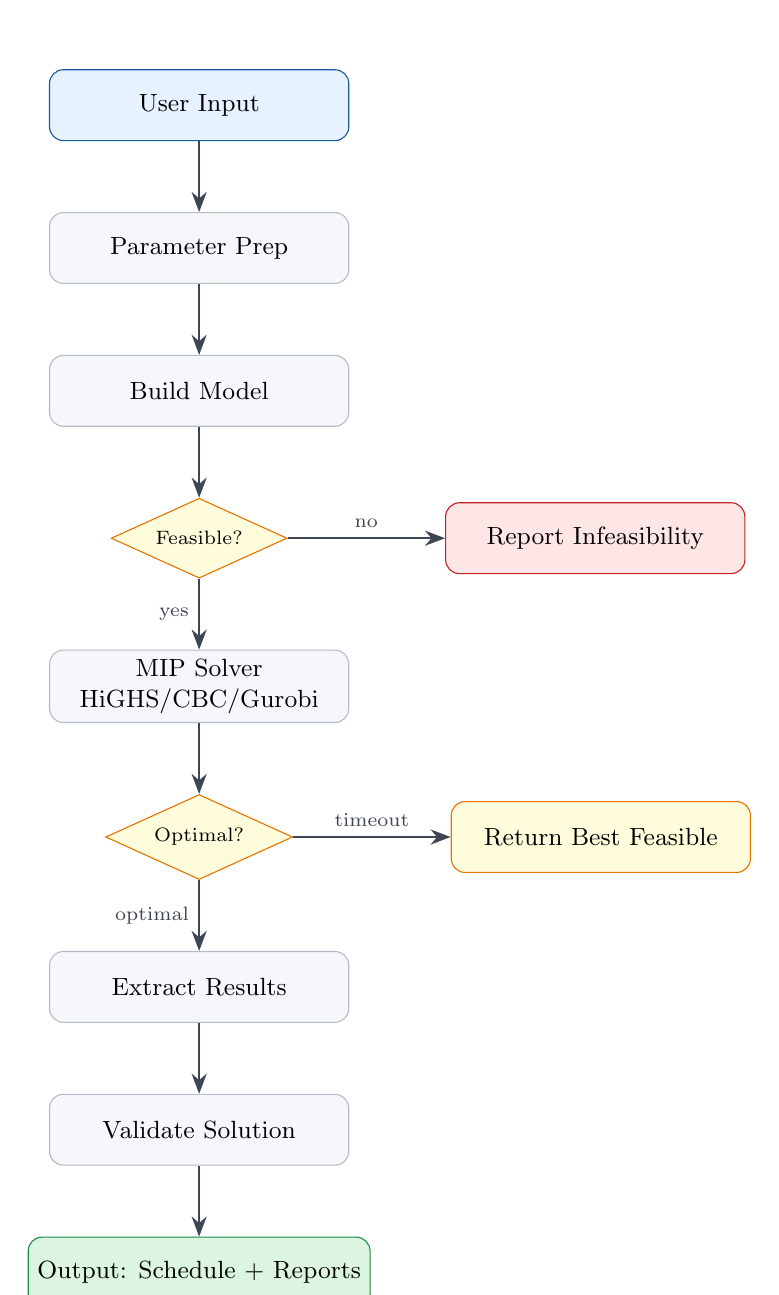
\begin{tikzpicture}[
  node distance=0.9cm and 2.2cm,
  block/.style={draw, rounded corners=5pt, fill=softgray, draw=midgray,
                minimum width=3.8cm, minimum height=0.9cm,
                font=\small, text centered, align=center},
  decision/.style={draw, diamond, aspect=2.2, fill=paleyellow, draw=accentorange,
                   font=\scriptsize, text centered},
  arrow/.style={-{Stealth[scale=1.1]}, thick, color=darkgray},
  label/.style={font=\scriptsize, color=darkgray}
]

  \node[block, fill=paleblue, draw=royalblue] (input) {User Input};
  \node[block, below=of input] (param)  {Parameter Prep};
  \node[block, below=of param] (build)  {Build Model};
  \node[decision, below=of build] (feas) {Feasible?};
  \node[block, right=2cm of feas, fill=palered, draw=accentred] (infeas) {Report Infeasibility};
  \node[block, below=of feas] (solve)  {MIP Solver\\HiGHS/CBC/Gurobi};
  \node[decision, below=of solve] (opt) {Optimal?};
  \node[block, right=2cm of opt, fill=paleyellow, draw=accentorange] (subopt) {Return Best Feasible};
  \node[block, below=of opt] (extract) {Extract Results};
  \node[block, below=of extract] (valid) {Validate Solution};
  \node[block, below=of valid, fill=palegreen, draw=accentgreen] (output) {Output: Schedule + Reports};

  \draw[arrow] (input) -- (param);
  \draw[arrow] (param) -- (build);
  \draw[arrow] (build) -- (feas);
  \draw[arrow] (feas) -- node[label, left]{yes} (solve);
  \draw[arrow] (feas) -- node[label, above]{no} (infeas);
  \draw[arrow] (solve) -- (opt);
  \draw[arrow] (opt) -- node[label, left]{optimal} (extract);
  \draw[arrow] (opt) -- node[label, above]{timeout} (subopt);
  \draw[arrow] (extract) -- (valid);
  \draw[arrow] (valid) -- (output);
\end{tikzpicture}
\end{center}

\subsection{Core Mathematical Flow}

\textbf{Decision Variables:}
\begin{align}
  sr_{ijk}, so_{ijk} &\in \{0,1\} & &\text{Regular / overtime shift assignment}\\
  \alpha_{jk}^{\omega} &\geq 0 & &\text{Emergency staff added (scenario }\omega)\\
  \beta_{jk}^{\omega} &\geq 0 & &\text{Shifts cancelled (scenario }\omega)
\end{align}

\textbf{Objective:}
\begin{eqbox}
\begin{equation}
  \min\;
  \underbrace{c_1 \textstyle\sum sr_{ijk} + c_2\sum so_{ijk}}_{\text{Stage 1}}
  +\underbrace{\mathbb{E}\bigl[q^{+}\alpha + q^{-}\beta\bigr]}_{\text{Stage 2 expected}}
\end{equation}
\end{eqbox}

\textbf{Optional CVaR Risk Control:}
\begin{equation}
  \text{CVaR}_{95\%}
  = \xi + \frac{1}{1-0.95}\sum_{\omega} p^{\omega}\, z^{\omega} \leq \mu,
  \qquad z^{\omega} = \max\!\Bigl(0,\textstyle\sum\alpha_{jk}^{\omega}-\xi\Bigr)
\end{equation}

\newpage
% ─────────────────────────────────────────────────────────────────────────────
%  SECTION 5 · CODE DYNAMICS FLOWCHART
% ─────────────────────────────────────────────────────────────────────────────
\section{Code Structure \& Dynamics}

\subsection{File Organisation}

\begin{center}
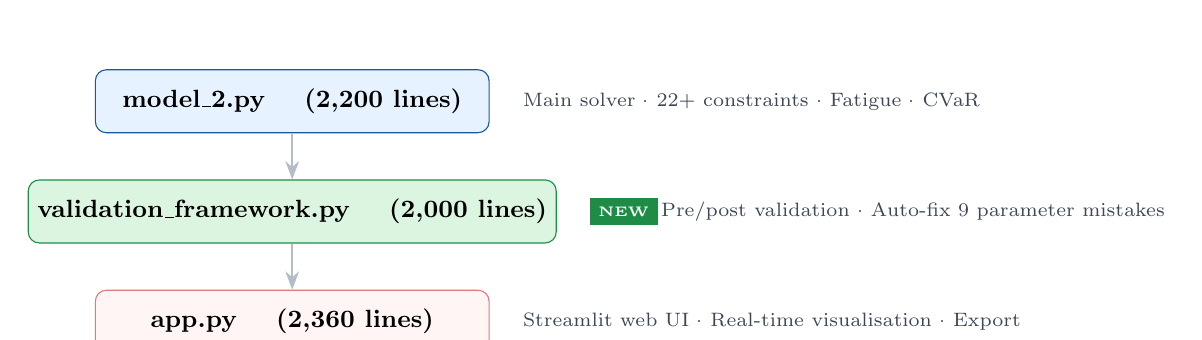
\begin{tikzpicture}[
  file/.style={draw, rounded corners=4pt, fill=softgray, draw=midgray,
               minimum width=5cm, minimum height=0.8cm,
               font=\small\bfseries, text centered},
  desc/.style={font=\scriptsize, color=darkgray, align=left},
  arrow/.style={-{Stealth}, thick, color=midgray}
]
  \node[file, fill=paleblue, draw=royalblue] (m2) at (0,0) {model\_2.py \quad\small(2,200 lines)};
  \node[desc, right=0.3cm of m2] {Main solver · 22+ constraints · Fatigue · CVaR};

  \node[file, fill=palegreen, draw=accentgreen] (vf) at (0,-1.4) {validation\_framework.py \quad\small(2,000 lines)};
  \node[desc, right=0.3cm of vf] {\newbadge Pre/post validation · Auto-fix 9 parameter mistakes};

  \node[file, fill=palered!40, draw=accentred!60] (app) at (0,-2.8) {app.py \quad\small(2,360 lines)};
  \node[desc, right=0.3cm of app] {Streamlit web UI · Real-time visualisation · Export};

  \draw[arrow] (m2) -- (vf);
  \draw[arrow] (vf) -- (app);
\end{tikzpicture}
\end{center}

\subsection{Execution Flow}

\begin{enumerate}[leftmargin=20pt, itemsep=8pt,
    label=\colorbox{navyblue}{\color{white}\small\bfseries\arabic*.}]

  \item \textbf{User Input} — The user provides everything the model needs to run:
    \begin{itemize}[itemsep=3pt]
      \item The list of nurses available for scheduling.
      \item Demand scenarios — each scenario says ``on day $j$, shift $k$, we expect $R$ nurses to be needed.'' Multiple scenarios represent different possible futures (e.g.\ a quiet week vs.\ a busy flu season).
      \item Cost parameters: $c_1$ (regular shift cost), $c_2$ (overtime cost), $q^+$ (emergency staff cost), $q^-$ (cancellation cost). The model will not work correctly unless $c_1 < c_2 < q^+$ — regular must be cheapest, emergency most expensive.
      \item Work rules: how many total shifts each nurse can work ($n_1$), how many night shifts are allowed ($n_2$), how many must be regular vs.\ overtime ($n_3$), and how many full weekends off are required ($n_4$).
      \item Model type: plain cost minimisation (SDM) or risk-aware with CVaR (SDM-CVaR).
    \end{itemize}

  \item \textbf{Validation} — Before building anything, the code runs four checks to catch mistakes early:
    \begin{itemize}[itemsep=3pt]
      \item \textit{Data structure check} — are all required columns present? Are nurse IDs unique? Are scenario labels consistent across days and shifts?
      \item \textit{Parameter range check} — is the cost hierarchy correct ($c_1 < c_2 < q^+$)? Are work-rule parameters consistent with each other (e.g.\ $n_1 \geq n_3$)?
      \item \textit{Capacity feasibility check} — can the nurses physically cover the demand, even in the worst case? If a hard cap on emergency staff is set and demand still cannot be met, the model will never find a solution, so this is caught here before wasting time solving.
      \item \textit{Problem-size estimation} — the code estimates how many variables and constraints the model will have, and how long it is likely to take to solve. A 30-nurse, 30-day problem with 20 scenarios has around 72,000 variables. This step warns the user if the problem is unusually large.
    \end{itemize}

  \item \textbf{Parameter Preparation} — Some parameters can be automatically derived so the user does not have to set everything manually. For example, if the user does not specify $n_1$ (max total shifts), the code sets it based on the length of the planning horizon. $n_2$ (max night shifts) defaults to roughly 30\% of $n_1$. Any value the user explicitly provided overrides the automatic one.

  \item \textbf{Model Building} — This is where the mathematical model is assembled inside the solver. The code creates all decision variables:
    \begin{itemize}[itemsep=3pt]
      \item $sr_{ijk}$ and $so_{ijk}$ — binary variables for regular and overtime shifts.
      \item $\alpha_{jk}^{\omega}$ and $\beta_{jk}^{\omega}$ — integer variables for emergency additions and cancellations in each scenario.
      \item $F_{ij}$, $w_{ij}$, $fw_{ij}$ — continuous and binary variables for fatigue tracking.
      \item $\xi$ and $z^{\omega}$ — variables for CVaR risk control (only if SDM-CVaR mode is selected).
    \end{itemize}
    It then adds all constraints (work rules, demand coverage, fatigue dynamics, CVaR bounds) and sets up the objective function. Finally, it selects the best available solver — HiGHS is preferred if installed, then CBC, then Gurobi if a license is available.

  \item \textbf{Solving} — The solver runs a branch-and-cut algorithm, which is the standard method for mixed-integer programming. It explores possible schedules by branching on binary decisions (``does nurse $i$ work on day $j$?'') and cuts off branches that cannot improve the current best solution. The time limit and acceptable optimality gap are scaled automatically based on problem size — a small problem gets a tight gap, a large problem may be stopped early and return the best solution found so far.

  \item \textbf{Result Extraction} — Once the solver finishes, the code reads the values of all decision variables and organises them into useful outputs:
    \begin{itemize}[itemsep=3pt]
      \item A schedule table showing which nurse works which shift on which day.
      \item A cost breakdown: how much came from regular shifts, overtime, emergency staff, cancellations, soft penalties, and fatigue costs.
      \item Risk metrics: if CVaR was used, the worst-case shortage and the CVaR value are reported.
      \item Scenario analysis: for each demand scenario, how many emergency staff were needed and at what cost.
    \end{itemize}

  \item \textbf{Solution Validation} — The code runs a second round of checks on the solution itself:
    \begin{itemize}[itemsep=3pt]
      \item Did the solver confirm the solution is optimal, or did it time out?
      \item Does the schedule respect all hard constraints — one shift per nurse per day, max total shifts, max night shifts?
      \item Is the reported cost consistent with what you get if you manually add up the assigned shifts?
    \end{itemize}
    This step exists because solver outputs can occasionally contain numerical errors or be misread. Catching them here prevents wrong results from being reported.

  \item \textbf{Output} — The final results are delivered to the user in three ways:
    \begin{itemize}[itemsep=3pt]
      \item An interactive web dashboard (built with Streamlit) showing the schedule, charts, and cost breakdown.
      \item Exportable files in CSV and JSON format for use in other tools or for sharing.
      \item Reproducibility metadata — a record of every parameter used, the solver settings, the random seed, and the result, so the exact same run can be repeated later.
    \end{itemize}

\end{enumerate}

\newpage
% ─────────────────────────────────────────────────────────────────────────────
%  SECTION 6 · COMPLETE MATHEMATICAL MODEL
% ─────────────────────────────────────────────────────────────────────────────
\section{Complete Mathematical Formulation}

\subsection{Decision Variables}

\begin{center}
\begin{tabularx}{\textwidth}{@{}llX@{}}
  \toprule
  \textbf{Variable} & \textbf{Domain} & \textbf{Meaning}\\
  \midrule
  $sr_{ijk}$         & $\{0,1\}$          & Regular shift — nurse $i$, day $j$, shift $k$\\
  $so_{ijk}$         & $\{0,1\}$          & Overtime shift\\
  $SR_i, SO_i$       & $\{0,1\}$          & Indicator: nurse works any regular/overtime shift\\
  $\alpha_{jk}^{\omega}$ & $\mathbb{Z}_{\geq 0}$ & Emergency staff added (scenario $\omega$)\\
  $\beta_{jk}^{\omega}$  & $\mathbb{Z}_{\geq 0}$ & Shifts cancelled (scenario $\omega$)\\
  $dev1_{ij}$        & $\mathbb{Z}_{\geq 0}$ & Stand-alone shift penalty (soft)\\
  $dev2_{ijk}$       & $\mathbb{Z}_{\geq 0}$ & Unwanted pattern penalty (soft)\\
  \rowcolor{palegreen}
  $F_{ij}$           & $[0,F_{\max}]$     & Cumulative fatigue level for nurse $i$ on day $j$ \contribbadge\\
  \rowcolor{palegreen}
  $w_{ij}$           & $\{0,1\}$          & Binary: 1 if nurse $i$ works any shift on day $j$ \contribbadge\\
  \rowcolor{palegreen}
  $fw_{ij}$          & $[0,F_{\max}]$     & McCormick auxiliary: equals $F_{i,j-1}\times w_{ij}$ \contribbadge\\
  $\xi$              & $\mathbb{R}$       & Value-at-Risk threshold (CVaR)\\
  $z^{\omega}$       & $\mathbb{R}_{\geq 0}$ & Excess loss in scenario $\omega$\\
  \bottomrule
\end{tabularx}
\end{center}

\subsection{Objective Function}

\begin{eqbox}
\begin{align}
  \min\;
  &\underbrace{c_1 \sum_i\sum_j\sum_k sr_{ijk}
  + c_2 \sum_i\sum_j\sum_k so_{ijk}}_{\text{Stage 1: Baseline Cost}}
  \notag\\[6pt]
  +\;&\underbrace{c_3 \sum_i\sum_j dev1_{ij}
  + c_4 \sum_i\sum_j\sum_k dev2_{ijk}}_{\text{Soft Constraint Penalties}}
  \notag\\[6pt]
  +\;&\underbrace{\sum_{\omega} p^{\omega}
    \Bigl(q^{+}\sum_j\sum_k\alpha_{jk}^{\omega}
         +q^{-}\sum_j\sum_k\beta_{jk}^{\omega}\Bigr)
  }_{\text{Stage 2: Expected Recourse Cost}}
  \notag\\[6pt]
  +\;&\underbrace{c_{\text{safety}}\sum_i\sum_j F_{ij}
  }_{\textcolor{accentred}{\textbf{Our Contribution: Fatigue Cost}}}
\end{align}
\end{eqbox}

\newpage
\subsection{Constraints}

\subsubsection{Core Constraints \frombadge (He et al., 2019)}

\begin{align}
  \sum_k (sr_{ijk}+so_{ijk}) &\leq 1 \quad \forall i,j
    && \text{(C1: one shift/day)}\\
  \sum_{j,k}(sr_{ijk}+so_{ijk}) &\leq n_1 \quad \forall i
    && \text{(C6: max total shifts)}\\
  \sum_j(sr_{ijN}+so_{ijN}) &\leq n_2 \quad \forall i
    && \text{(C7: max night shifts)}\\
  \sum_i(sr_{ijk}+so_{ijk})+\alpha_{jk}^{\omega}-\beta_{jk}^{\omega}
    &\geq R_{jk}^{\omega} \quad \forall j,k,\omega
    && \text{(C16: demand fulfillment)}
\end{align}

\subsubsection{Our Constraint Modifications \modbadge / \newbadge}

\begin{eqbox}
\textbf{C8 — Regular Shift Quota} \modbadge
\begin{equation}
  \textcolor{accentred}{\sum_{j,k} sr_{ijk} = n_3 \cdot SR_i \quad \forall i}
  \qquad\text{(strict equality; paper uses $\geq$)}
\end{equation}
\end{eqbox}

\vspace{6pt}
\begin{eqbox}
\textbf{C7.5 — Weekly Overtime Cap} \newbadge
\begin{equation}
  \textcolor{accentred}{\sum_{j \in \text{week}\,w}\sum_k so_{ijk} \leq 1 \quad \forall i,w}
\end{equation}
\end{eqbox}

\vspace{6pt}
\begin{eqbox}
\textbf{C2–C5 — Shift-Type Quotas} \newbadge
\begin{equation}
  \textcolor{accentred}{
    n_{k,\min} \leq \sum_j(sr_{ijk}+so_{ijk}) \leq n_{k,\max}
    \quad \forall i,\; k \in \{E,D,L,N\}
  }
\end{equation}
\end{eqbox}

\vspace{6pt}
\begin{eqbox}
\textbf{C9 — Minimum Complete Weekends Off} \newbadge
\begin{equation}
  \textcolor{accentred}{\sum_w \text{weekend\_off}_{iw} \geq n_4 \quad \forall i}
\end{equation}
\end{eqbox}

\subsubsection{Fatigue Constraints \contribbadge}

\begin{eqbox}
\textbf{Work indicator — $w_{i,j}$} (binary helper: 1 if nurse $i$ works any shift on day $j$)
\begin{equation}
  \textcolor{accentred}{
    w_{i,j} \geq \textstyle\sum_k(sr_{ijk}+so_{ijk}), \qquad
    w_{i,j} \leq \textstyle\sum_k(sr_{ijk}+so_{ijk}) \quad \forall i,j
  }
\end{equation}

\textbf{F-MC — McCormick auxiliary variable $fw_{i,j}$} (linearises $F_{i,j-1}\times w_{i,j}$)
\begin{align}
  \textcolor{accentred}{fw_{i,j}} &\textcolor{accentred}{\leq M \cdot w_{i,j}} \tag{MC1}\\
  \textcolor{accentred}{fw_{i,j}} &\textcolor{accentred}{\leq F_{i,j-1}} \tag{MC2}\\
  \textcolor{accentred}{fw_{i,j}} &\textcolor{accentred}{\geq F_{i,j-1} - M(1-w_{i,j})} \tag{MC3}\\
  \textcolor{accentred}{fw_{i,j}} &\textcolor{accentred}{\geq 0} \tag{MC4}
\end{align}
where $M = F_{\max} = 0.70$.

\textbf{F1 — Fatigue Dynamics} (one linear equation covers both work and rest days)
\begin{equation}
  \textcolor{accentred}{
    F_{i,j} = F_{i,j-1}\cdot d_{\text{off}}
    + (d_{\text{work}}-d_{\text{off}})\cdot fw_{i,j}
    + \Delta_f \cdot w_{i,j}
    \quad\forall i,j
  }
\end{equation}

\textbf{F2 — Fatigue Upper Bound}
\begin{equation}
  \textcolor{accentred}{F_{i,j} \leq F_{\max} \quad \forall i,j}
\end{equation}
\end{eqbox}

\subsubsection{CVaR Risk Control \frombadge}

\begin{eqbox}
\textbf{C19 — CVaR Upper Bound}
\begin{equation}
  \xi + \frac{1}{1-\sigma}\sum_{\omega} p^{\omega}\, z^{\omega} \leq \mu
\end{equation}

\textbf{C22 — Excess Loss Definition}
\begin{equation}
  z^{\omega} \geq \sum_j\sum_k \alpha_{jk}^{\omega} - \xi \quad \forall\omega
\end{equation}
\end{eqbox}

\newpage
% ─────────────────────────────────────────────────────────────────────────────
%  SECTION 8 · WHAT NEEDS TO BE DONE BEFORE PUBLICATION
% ─────────────────────────────────────────────────────────────────────────────
\section{What Needs to Be Done Before Publication}

This section is honest about the current state of the work. The model is built and runs correctly, but there are several steps required before it can be considered validated and ready for a research paper.

\subsection{Critical Tasks}

\begin{warnbox}[Task 1 — Check If the Fatigue Framework is Realistic]
\textbf{The problem:} The fatigue parameters we use ($\lambda=0.03$, $F_{\max}=0.70$) were taken from a study on \emph{factory assembly workers}, not nurses. Nurses have very different working conditions. If these numbers are wrong, then the entire fatigue cost term in our model is not meaningful.

\textbf{What we need to do:}
\begin{itemize}[itemsep=2pt]
  \item Get access to real hospital data that links nurse shift history to medical error rates.
  \item Use that data to find the correct values of $\lambda$ and $F_{\max}$ for nurses specifically.
  \item Re-run the model with the corrected values and verify the fatigue dynamics still behave as expected.
\end{itemize}

\textbf{Why it matters:} Without this, a reviewer can (correctly) say our safety model has no clinical basis.\\
\end{warnbox}

\vspace{6pt}
\begin{warnbox}[Task 2 — Get Real Hospital Data]
\textbf{The problem:} Right now we are testing the model on \textbf{synthetic (made-up) data}. This is our last resort — we use it because we have no real data yet. Synthetic data lets us confirm the model works mathematically, but it does not prove it would work in a real hospital.

\textbf{What real data looks like:}
\begin{itemize}[itemsep=2pt]
  \item Daily patient admission numbers over at least 90 days.
  \item Which department each patient went to (ICU, ER, general ward, etc.) — because each department needs a different number of nurses.
  \item The actual shift schedules the hospital used during that same period.
  \item Any recorded incidents: patient safety events, overtime complaints, under-staffing flags.
\end{itemize}

\textbf{What we do with it:} We run our model on the historical data as if we were planning the schedule from scratch, then compare our suggested schedule to what the hospital actually did. If our schedule is cheaper and equally safe, that is a strong result.

\textbf{Why it matters:} A paper based only on synthetic data will be difficult to publish in a high-quality operations or healthcare journal.\\
\end{warnbox}

\vspace{6pt}
\begin{warnbox}[Task 3 — Test the Model Against Real History (if applicable)]
\textbf{Depends on:} Task 2 (real data) must be completed first.\\[4pt]
\textbf{What we do:}
\begin{enumerate}[itemsep=2pt]
  \item Feed the model 6 months (for example) of historical data and let it build a schedule.
  \item Compare our schedule to what the hospital actually did over the same 6 months.
  \item Measure the difference in cost, staffing coverage, and safety incidents.
  \item If the gap is less than 5\% (for example), we have a publishable result.
\end{enumerate}
\textbf{Why it matters:} This is the main experiment of the paper. Everything else builds toward this test.
\end{warnbox}

\subsection{Current Weak Points}

\begin{warnbox}[Known Limitations to Acknowledge]
\begin{itemize}[itemsep=6pt]
  \item \textbf{Fatigue parameters from a different domain} — We borrowed industrial worker values. Until we recalibrate for nurses, we should present the fatigue model as a structural contribution, not a clinically validated one. Run a sensitivity analysis ($\pm50\%$ on $\lambda$) to show the model's behaviour across a range of values.

  \item \textbf{Currently using synthetic data} — This is our fallback while we wait for hospital access. We should clearly state this in the paper and frame it as: ``results demonstrate proof-of-concept; real-data validation is planned.''

  \item \textbf{All nurses are treated as equal} — In reality, an ICU nurse and a general-ward nurse are not interchangeable. Our model currently assigns any nurse to any shift. This is a known simplification.

  \item \textbf{Solver speed at large scale} — The model handles 30 nurses over 30 days in 1–5 minutes. If the hospital has 100+ nurses, solve time could reach 30–60 minutes, which is too slow for daily re-planning. We should acknowledge this and mention decomposition methods as future work.

  \item \textbf{Nurse preferences are ignored} — The model does not factor in whether a nurse prefers morning shifts or has requested days off. This may reduce how willing nurses are to accept the generated schedules.
\end{itemize}
\end{warnbox}

\newpage
\subsection{Validation Timeline}

\begin{center}
\begin{tabular}{lccc}
  \toprule
  \textbf{Task} & \textbf{Estimated Time} & \textbf{Required?} & \textbf{Status}\\
  \midrule
  Fatigue parameter calibration & 2–3 months & \textcolor{accentred}{\textbf{Yes}} & \colorbox{paleyellow}{\small In Progress}\\
  Real hospital demand data     & 3–6 months & \textcolor{accentred}{\textbf{Yes}} & \colorbox{palered}{\small Not Started}\\
  Clinical constraint review    & 4–8 weeks  & \textcolor{accentred}{\textbf{Yes}} & \colorbox{palered}{\small Not Started}\\
  Historical performance test   & 2–3 months & \textcolor{accentred}{\textbf{Yes}} & \colorbox{palered}{\small Blocked}\\
  \bottomrule
\end{tabular}
\end{center}

\subsection{Future Work (For the Paper's Future Work Section)}

The following ideas are \textbf{not planned for the current version} of the project, but they are worth stating in the paper to show where this research can go next.

\begin{solutionbox}[Skill-Based Nurse Assignment]
Currently all nurses are treated as having the same skills. A natural extension would be to add skill levels (e.g., ICU-certified, general ward, paediatric) and require that each shift is covered by nurses with the right qualifications. This would make the model much more applicable to real hospital deployments.
\end{solutionbox}

\vspace{6pt}
\begin{solutionbox}[Nurse Preferences and Work-Life Balance]
Adding a preference layer to the model — letting nurses flag preferred shifts or request days off — would make the schedule more acceptable in practice and reduce staff turnover. This can be implemented as a bonus term in the objective function.
\end{solutionbox}

\vspace{6pt}
\begin{solutionbox}[Better Demand Scenario Generation]
Right now demand scenarios are constructed manually or from simple proxies. A more rigorous approach would be to fit a statistical model to historical admission data and generate 500–1000 realistic scenarios automatically. This would make the CVaR constraints much more meaningful.
\end{solutionbox}

\newpage
% ─────────────────────────────────────────────────────────────────────────────
%  SECTION 9 · CONCLUSION
% ─────────────────────────────────────────────────────────────────────────────
\section{Conclusion}

FROST-NS started from a published nurse scheduling model (He et al., 2019) and extended it in four meaningful ways: we fixed a structural flaw in how overtime is handled, we introduced a piecewise-linear fatigue model that can actually be solved by standard optimisation software, we added seven new constraint types that reflect real hospital policies, and we built a validation framework that makes results reproducible and honest.

The model currently works correctly on synthetic data, which serves as proof-of-concept. \textbf{Synthetic data is our last resort} — it confirms the mathematics is sound, but it is not sufficient on its own for a strong publication. The critical next step is obtaining real patient demand data from a hospital and running the model against historical scheduling decisions. Combined with clinical input on the constraint parameters, this would transform the project from a well-built prototype into a validated, publishable contribution to healthcare operations research.

\begin{contribbox}[What We Have Built]
\begin{itemize}[itemsep=5pt]
  \item \textbf{A working two-stage stochastic MIP} that balances cost, risk, and nurse fatigue in a single model.
  \item \textbf{The first practical PWL fatigue implementation} for nurse scheduling — a contribution no prior paper has made in MIP form.
  \item \textbf{A corrected overtime mechanism} that fixes a known flaw in the base paper. (May Need Validation)
  \item \textbf{An honest validation framework} that reports what the model can and cannot do.
\end{itemize}
\end{contribbox}

\end{document}